\begin{figure}
\centering
%% Created by tikzDevice version 0.12.3.1 on 2022-11-04 11:05:01
% !TEX encoding = UTF-8 Unicode
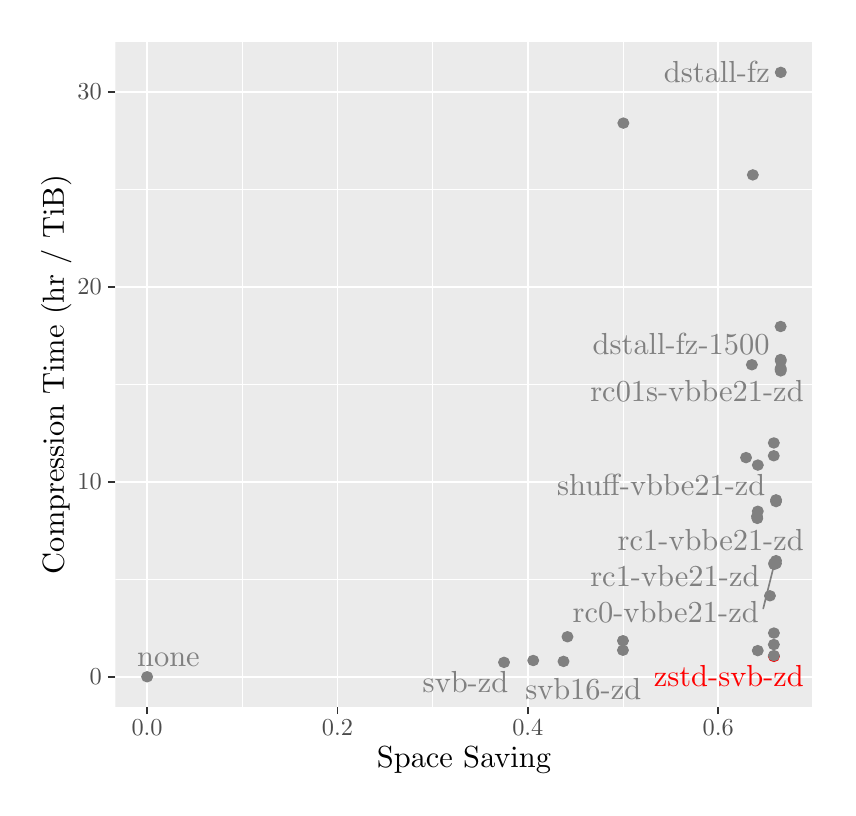
\begin{tikzpicture}[x=1pt,y=0.95pt]
\definecolor{fillColor}{RGB}{255,255,255}
\path[use as bounding box,fill=fillColor,fill opacity=0.00] (0,0) rectangle (289.08,289.08);
\begin{scope}
\path[clip] (  0.00,  0.00) rectangle (289.08,289.08);
\definecolor{drawColor}{RGB}{255,255,255}
\definecolor{fillColor}{RGB}{255,255,255}

\path[draw=drawColor,line width= 0.6pt,line join=round,line cap=round,fill=fillColor] (  0.00,  0.00) rectangle (289.08,289.08);
\end{scope}
\begin{scope}
\path[clip] ( 31.71, 30.69) rectangle (283.58,283.58);
\definecolor{fillColor}{gray}{0.92}

\path[fill=fillColor] ( 31.71, 30.69) rectangle (283.58,283.58);
\definecolor{drawColor}{RGB}{255,255,255}

\path[draw=drawColor,line width= 0.3pt,line join=round] ( 31.71, 79.26) --
	(283.58, 79.26);

\path[draw=drawColor,line width= 0.3pt,line join=round] ( 31.71,153.43) --
	(283.58,153.43);

\path[draw=drawColor,line width= 0.3pt,line join=round] ( 31.71,227.60) --
	(283.58,227.60);

\path[draw=drawColor,line width= 0.3pt,line join=round] ( 77.55, 30.69) --
	( 77.55,283.58);

\path[draw=drawColor,line width= 0.3pt,line join=round] (146.34, 30.69) --
	(146.34,283.58);

\path[draw=drawColor,line width= 0.3pt,line join=round] (215.13, 30.69) --
	(215.13,283.58);

\path[draw=drawColor,line width= 0.6pt,line join=round] ( 31.71, 42.18) --
	(283.58, 42.18);

\path[draw=drawColor,line width= 0.6pt,line join=round] ( 31.71,116.35) --
	(283.58,116.35);

\path[draw=drawColor,line width= 0.6pt,line join=round] ( 31.71,190.51) --
	(283.58,190.51);

\path[draw=drawColor,line width= 0.6pt,line join=round] ( 31.71,264.68) --
	(283.58,264.68);

\path[draw=drawColor,line width= 0.6pt,line join=round] ( 43.16, 30.69) --
	( 43.16,283.58);

\path[draw=drawColor,line width= 0.6pt,line join=round] (111.95, 30.69) --
	(111.95,283.58);

\path[draw=drawColor,line width= 0.6pt,line join=round] (180.73, 30.69) --
	(180.73,283.58);

\path[draw=drawColor,line width= 0.6pt,line join=round] (249.52, 30.69) --
	(249.52,283.58);
\definecolor{drawColor}{gray}{0.50}
\definecolor{fillColor}{gray}{0.50}

\path[draw=drawColor,line width= 0.4pt,line join=round,line cap=round,fill=fillColor] ( 43.16, 42.18) circle (  1.96);

\path[draw=drawColor,line width= 0.4pt,line join=round,line cap=round,fill=fillColor] (215.25,252.78) circle (  1.96);

\path[draw=drawColor,line width= 0.4pt,line join=round,line cap=round,fill=fillColor] (195.05, 57.40) circle (  1.96);

\path[draw=drawColor,line width= 0.4pt,line join=round,line cap=round,fill=fillColor] (262.03,233.08) circle (  1.96);

\path[draw=drawColor,line width= 0.4pt,line join=round,line cap=round,fill=fillColor] (172.13, 47.66) circle (  1.96);

\path[draw=drawColor,line width= 0.4pt,line join=round,line cap=round,fill=fillColor] (193.62, 48.03) circle (  1.96);

\path[draw=drawColor,line width= 0.4pt,line join=round,line cap=round,fill=fillColor] (182.68, 48.37) circle (  1.96);

\path[draw=drawColor,line width= 0.4pt,line join=round,line cap=round,fill=fillColor] (215.09, 52.28) circle (  1.96);

\path[draw=drawColor,line width= 0.4pt,line join=round,line cap=round,fill=fillColor] (215.10, 55.89) circle (  1.96);
\definecolor{drawColor}{RGB}{255,0,0}
\definecolor{fillColor}{RGB}{255,0,0}

\path[draw=drawColor,line width= 0.4pt,line join=round,line cap=round,fill=fillColor] (269.65, 49.93) circle (  1.96);
\definecolor{drawColor}{gray}{0.50}
\definecolor{fillColor}{gray}{0.50}

\path[draw=drawColor,line width= 0.4pt,line join=round,line cap=round,fill=fillColor] (269.64, 50.24) circle (  1.96);

\path[draw=drawColor,line width= 0.4pt,line join=round,line cap=round,fill=fillColor] (263.81, 52.13) circle (  1.96);

\path[draw=drawColor,line width= 0.4pt,line join=round,line cap=round,fill=fillColor] (269.63, 54.44) circle (  1.96);

\path[draw=drawColor,line width= 0.4pt,line join=round,line cap=round,fill=fillColor] (269.65, 58.81) circle (  1.96);

\path[draw=drawColor,line width= 0.4pt,line join=round,line cap=round,fill=fillColor] (263.53,103.18) circle (  1.96);

\path[draw=drawColor,line width= 0.4pt,line join=round,line cap=round,fill=fillColor] (263.65,102.42) circle (  1.96);

\path[draw=drawColor,line width= 0.4pt,line join=round,line cap=round,fill=fillColor] (259.58,125.54) circle (  1.96);

\path[draw=drawColor,line width= 0.4pt,line join=round,line cap=round,fill=fillColor] (263.83,105.14) circle (  1.96);

\path[draw=drawColor,line width= 0.4pt,line join=round,line cap=round,fill=fillColor] (263.84,122.70) circle (  1.96);

\path[draw=drawColor,line width= 0.4pt,line join=round,line cap=round,fill=fillColor] (261.69,160.86) circle (  1.96);

\path[draw=drawColor,line width= 0.4pt,line join=round,line cap=round,fill=fillColor] (268.22, 72.98) circle (  1.96);

\path[draw=drawColor,line width= 0.4pt,line join=round,line cap=round,fill=fillColor] (269.60,126.24) circle (  1.96);

\path[draw=drawColor,line width= 0.4pt,line join=round,line cap=round,fill=fillColor] (270.42,108.81) circle (  1.96);

\path[draw=drawColor,line width= 0.4pt,line join=round,line cap=round,fill=fillColor] (269.74, 85.41) circle (  1.96);

\path[draw=drawColor,line width= 0.4pt,line join=round,line cap=round,fill=fillColor] (270.40, 85.28) circle (  1.96);

\path[draw=drawColor,line width= 0.4pt,line join=round,line cap=round,fill=fillColor] (272.10,159.58) circle (  1.96);

\path[draw=drawColor,line width= 0.4pt,line join=round,line cap=round,fill=fillColor] (269.62,131.13) circle (  1.96);

\path[draw=drawColor,line width= 0.4pt,line join=round,line cap=round,fill=fillColor] (270.43,109.48) circle (  1.96);

\path[draw=drawColor,line width= 0.4pt,line join=round,line cap=round,fill=fillColor] (269.75, 84.94) circle (  1.96);

\path[draw=drawColor,line width= 0.4pt,line join=round,line cap=round,fill=fillColor] (270.42, 86.35) circle (  1.96);

\path[draw=drawColor,line width= 0.4pt,line join=round,line cap=round,fill=fillColor] (272.12,158.53) circle (  1.96);

\path[draw=drawColor,line width= 0.4pt,line join=round,line cap=round,fill=fillColor] (272.11,162.86) circle (  1.96);

\path[draw=drawColor,line width= 0.4pt,line join=round,line cap=round,fill=fillColor] (272.08,175.41) circle (  1.96);

\path[draw=drawColor,line width= 0.4pt,line join=round,line cap=round,fill=fillColor] (272.09,159.13) circle (  1.96);

\path[draw=drawColor,line width= 0.4pt,line join=round,line cap=round,fill=fillColor] (272.13,272.08) circle (  1.96);

\path[draw=drawColor,line width= 0.4pt,line join=round,line cap=round,fill=fillColor] (272.13,162.28) circle (  1.96);

\path[draw=drawColor,line width= 0.6pt,line join=round,line cap=round] (265.79, 68.14) -- (269.54, 84.04);

\node[text=drawColor,anchor=base,inner sep=0pt, outer sep=0pt, scale=  1.10] at ( 50.88, 46.14) {none};

\node[text=drawColor,anchor=base,inner sep=0pt, outer sep=0pt, scale=  1.10] at (158.22, 36.13) {svb-zd};

\node[text=drawColor,anchor=base,inner sep=0pt, outer sep=0pt, scale=  1.10] at (200.76, 33.70) {svb16-zd};
\definecolor{drawColor}{RGB}{255,0,0}

\node[text=drawColor,anchor=base,inner sep=0pt, outer sep=0pt, scale=  1.10] at (253.37, 38.38) {zstd-svb-zd};
\definecolor{drawColor}{gray}{0.50}

\node[text=drawColor,anchor=base,inner sep=0pt, outer sep=0pt, scale=  1.10] at (233.88, 76.64) {rc1-vbe21-zd};

\node[text=drawColor,anchor=base,inner sep=0pt, outer sep=0pt, scale=  1.10] at (228.96,111.12) {shuff-vbbe21-zd};

\node[text=drawColor,anchor=base,inner sep=0pt, outer sep=0pt, scale=  1.10] at (230.55, 62.88) {rc0-vbbe21-zd};

\node[text=drawColor,anchor=base,inner sep=0pt, outer sep=0pt, scale=  1.10] at (246.83, 90.28) {rc1-vbbe21-zd};

\node[text=drawColor,anchor=base,inner sep=0pt, outer sep=0pt, scale=  1.10] at (241.86,147.01) {rc01s-vbbe21-zd};

\node[text=drawColor,anchor=base,inner sep=0pt, outer sep=0pt, scale=  1.10] at (249.05,268.28) {dstall-fz};

\node[text=drawColor,anchor=base,inner sep=0pt, outer sep=0pt, scale=  1.10] at (236.11,164.81) {dstall-fz-1500};
\end{scope}
\begin{scope}
\path[clip] (  0.00,  0.00) rectangle (289.08,289.08);
\definecolor{drawColor}{gray}{0.30}

\node[text=drawColor,anchor=base east,inner sep=0pt, outer sep=0pt, scale=  0.88] at ( 26.76, 39.15) {0};

\node[text=drawColor,anchor=base east,inner sep=0pt, outer sep=0pt, scale=  0.88] at ( 26.76,113.32) {10};

\node[text=drawColor,anchor=base east,inner sep=0pt, outer sep=0pt, scale=  0.88] at ( 26.76,187.48) {20};

\node[text=drawColor,anchor=base east,inner sep=0pt, outer sep=0pt, scale=  0.88] at ( 26.76,261.65) {30};
\end{scope}
\begin{scope}
\path[clip] (  0.00,  0.00) rectangle (289.08,289.08);
\definecolor{drawColor}{gray}{0.20}

\path[draw=drawColor,line width= 0.6pt,line join=round] ( 28.96, 42.18) --
	( 31.71, 42.18);

\path[draw=drawColor,line width= 0.6pt,line join=round] ( 28.96,116.35) --
	( 31.71,116.35);

\path[draw=drawColor,line width= 0.6pt,line join=round] ( 28.96,190.51) --
	( 31.71,190.51);

\path[draw=drawColor,line width= 0.6pt,line join=round] ( 28.96,264.68) --
	( 31.71,264.68);
\end{scope}
\begin{scope}
\path[clip] (  0.00,  0.00) rectangle (289.08,289.08);
\definecolor{drawColor}{gray}{0.20}

\path[draw=drawColor,line width= 0.6pt,line join=round] ( 43.16, 27.94) --
	( 43.16, 30.69);

\path[draw=drawColor,line width= 0.6pt,line join=round] (111.95, 27.94) --
	(111.95, 30.69);

\path[draw=drawColor,line width= 0.6pt,line join=round] (180.73, 27.94) --
	(180.73, 30.69);

\path[draw=drawColor,line width= 0.6pt,line join=round] (249.52, 27.94) --
	(249.52, 30.69);
\end{scope}
\begin{scope}
\path[clip] (  0.00,  0.00) rectangle (289.08,289.08);
\definecolor{drawColor}{gray}{0.30}

\node[text=drawColor,anchor=base,inner sep=0pt, outer sep=0pt, scale=  0.88] at ( 43.16, 19.68) {0.0};

\node[text=drawColor,anchor=base,inner sep=0pt, outer sep=0pt, scale=  0.88] at (111.95, 19.68) {0.2};

\node[text=drawColor,anchor=base,inner sep=0pt, outer sep=0pt, scale=  0.88] at (180.73, 19.68) {0.4};

\node[text=drawColor,anchor=base,inner sep=0pt, outer sep=0pt, scale=  0.88] at (249.52, 19.68) {0.6};
\end{scope}
\begin{scope}
\path[clip] (  0.00,  0.00) rectangle (289.08,289.08);
\definecolor{drawColor}{RGB}{0,0,0}

\node[text=drawColor,anchor=base,inner sep=0pt, outer sep=0pt, scale=  1.10] at (157.65,  7.64) {Space Saving};
\end{scope}
\begin{scope}
\path[clip] (  0.00,  0.00) rectangle (289.08,289.08);
\definecolor{drawColor}{RGB}{0,0,0}

\node[text=drawColor,rotate= 90.00,anchor=base,inner sep=0pt, outer sep=0pt, scale=  1.10] at ( 13.08,157.13) {Compression Time (hr / TiB)};
\end{scope}
\end{tikzpicture}

\subfloat[\label{fig:results-ss-ct-big}]{
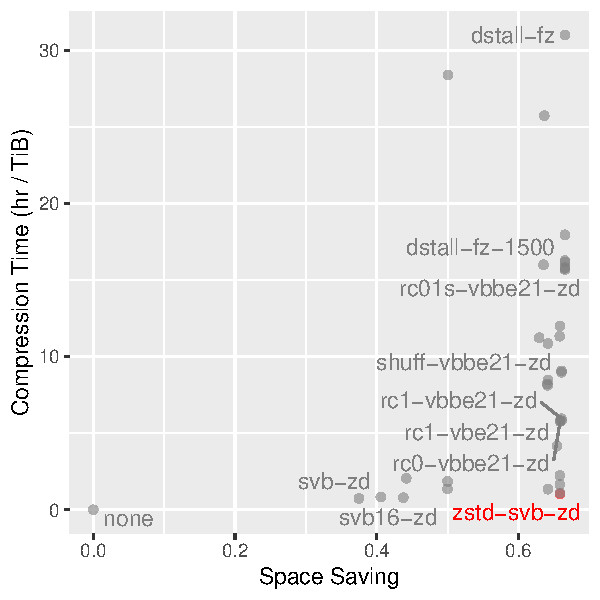
\includegraphics[scale=0.7,valign=t]{plots/reads.blow5.test.ss-ct.pdf}
}
\subfloat[\label{fig:results-ss-ct-small}]{
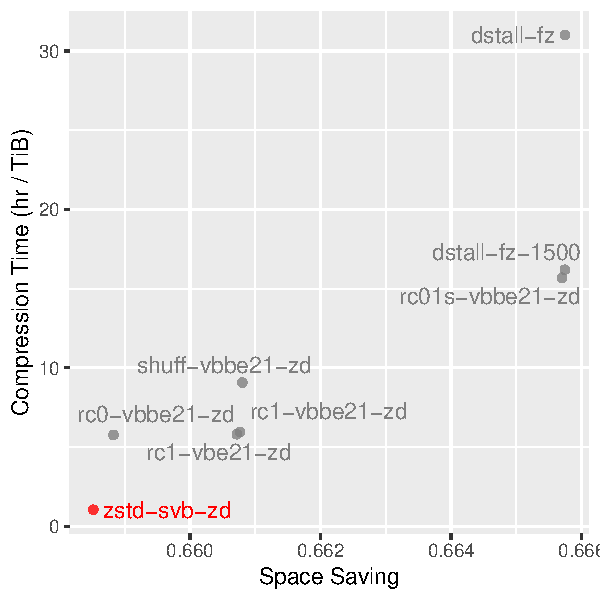
\includegraphics[scale=0.7,valign=t]{plots/reads.blow5.test.ss-ct06.pdf}
}

\subfloat[\label{fig:results-ss-dt-big}]{
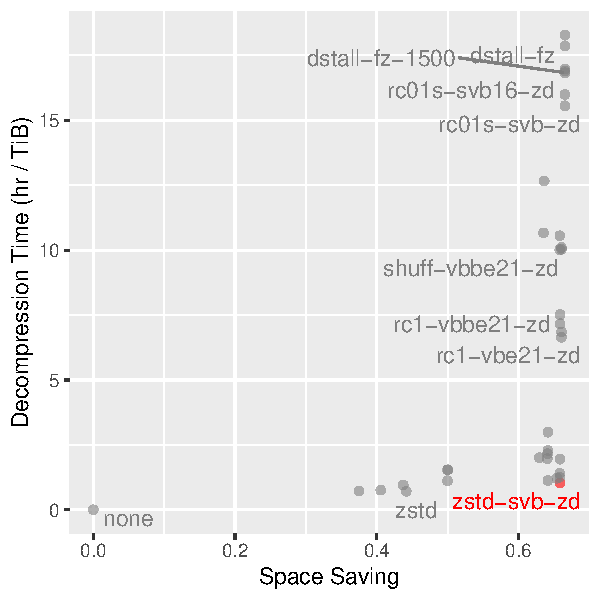
\includegraphics[scale=0.7,valign=t]{plots/reads.blow5.test.ss-dt.pdf}
}
\subfloat[\label{fig:results-ss-dt-small}]{
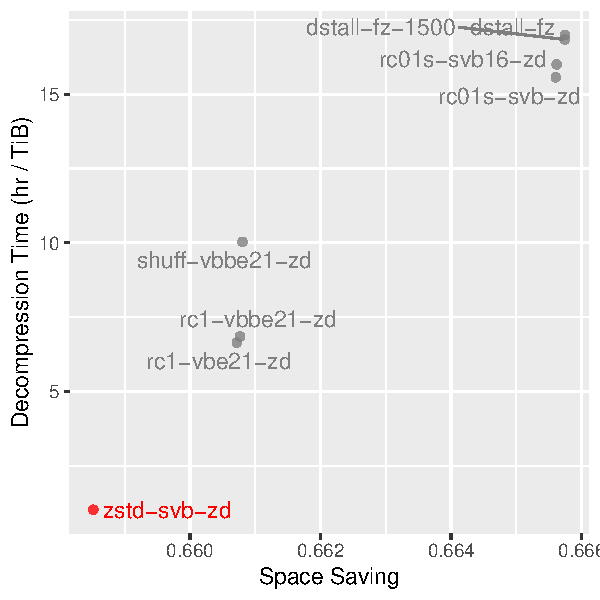
\includegraphics[scale=0.7,valign=t]{plots/reads.blow5.test.ss-dt06.pdf}
}
\caption{\label{fig:results-ss-t}The (de)compression time (in hours per TiB)
	versus space saving of various methods. The state-of-the-art method is
	coloured in red and the labelled methods are on the
	space--(de)compression-time frontier. That is, for each labelled method
	in Figures \ref{fig:results-ss-ct-big} and
	\ref{fig:results-ss-ct-small}
	there is no other compression method which produces a greater space
	saving in less time. Whilst for each labelled method in Figures
	\ref{fig:results-ss-dt-big} and \ref{fig:results-ss-dt-small} there is
	no other compression method which has a greater space saving and
	decompresses in less time.
	Figures \ref{fig:results-ss-ct-big} and \ref{fig:results-ss-dt-big} show all the
	methods. Whilst Figures \ref{fig:results-ss-ct-small} and
	\ref{fig:results-ss-dt-small} show the methods which are on their
	respective froniter and have a space saving greater than or equal to the
	state-of-the-art.}
\end{figure}
